\section{Data Description}

\begin{frame}{Data Description}
    \begin{itemize}
        \item Data was collected from about 3600 pages of PDFs from both the OBM website and from FOIA requests.
        \item There were a total of 43,596 projects listed in these PDFs
        \item Each project was scraped, the intersections of all roads were recorded and then located if they exist, and then located using the Census' geocoding API. If the census API failed, then Google Maps' API was used instead.
        \item In total, 83\% of the projects were successfully located using one of the two above methods.
        \item This dataset contains 41,381 precinct-year observations which record the total amount of spending in a given voting precinct in a given year.
    \end{itemize}
\end{frame}

\begin{frame}{PDF Example}
    \begin{figure}[H]
        \centering
        \includegraphics[width=0.6\textwidth]{input/menu_example2.png}
        \caption{Example of a Menu PDF}
        \label{fig:menu_example}
    \end{figure}
\end{frame}

\begin{frame}{Spending is quite concentrated}
    \begin{figure}[H]
        \centering
        % First subfigure
        \begin{subfigure}[b]{0.45\textwidth} % [b] aligns at the bottom
          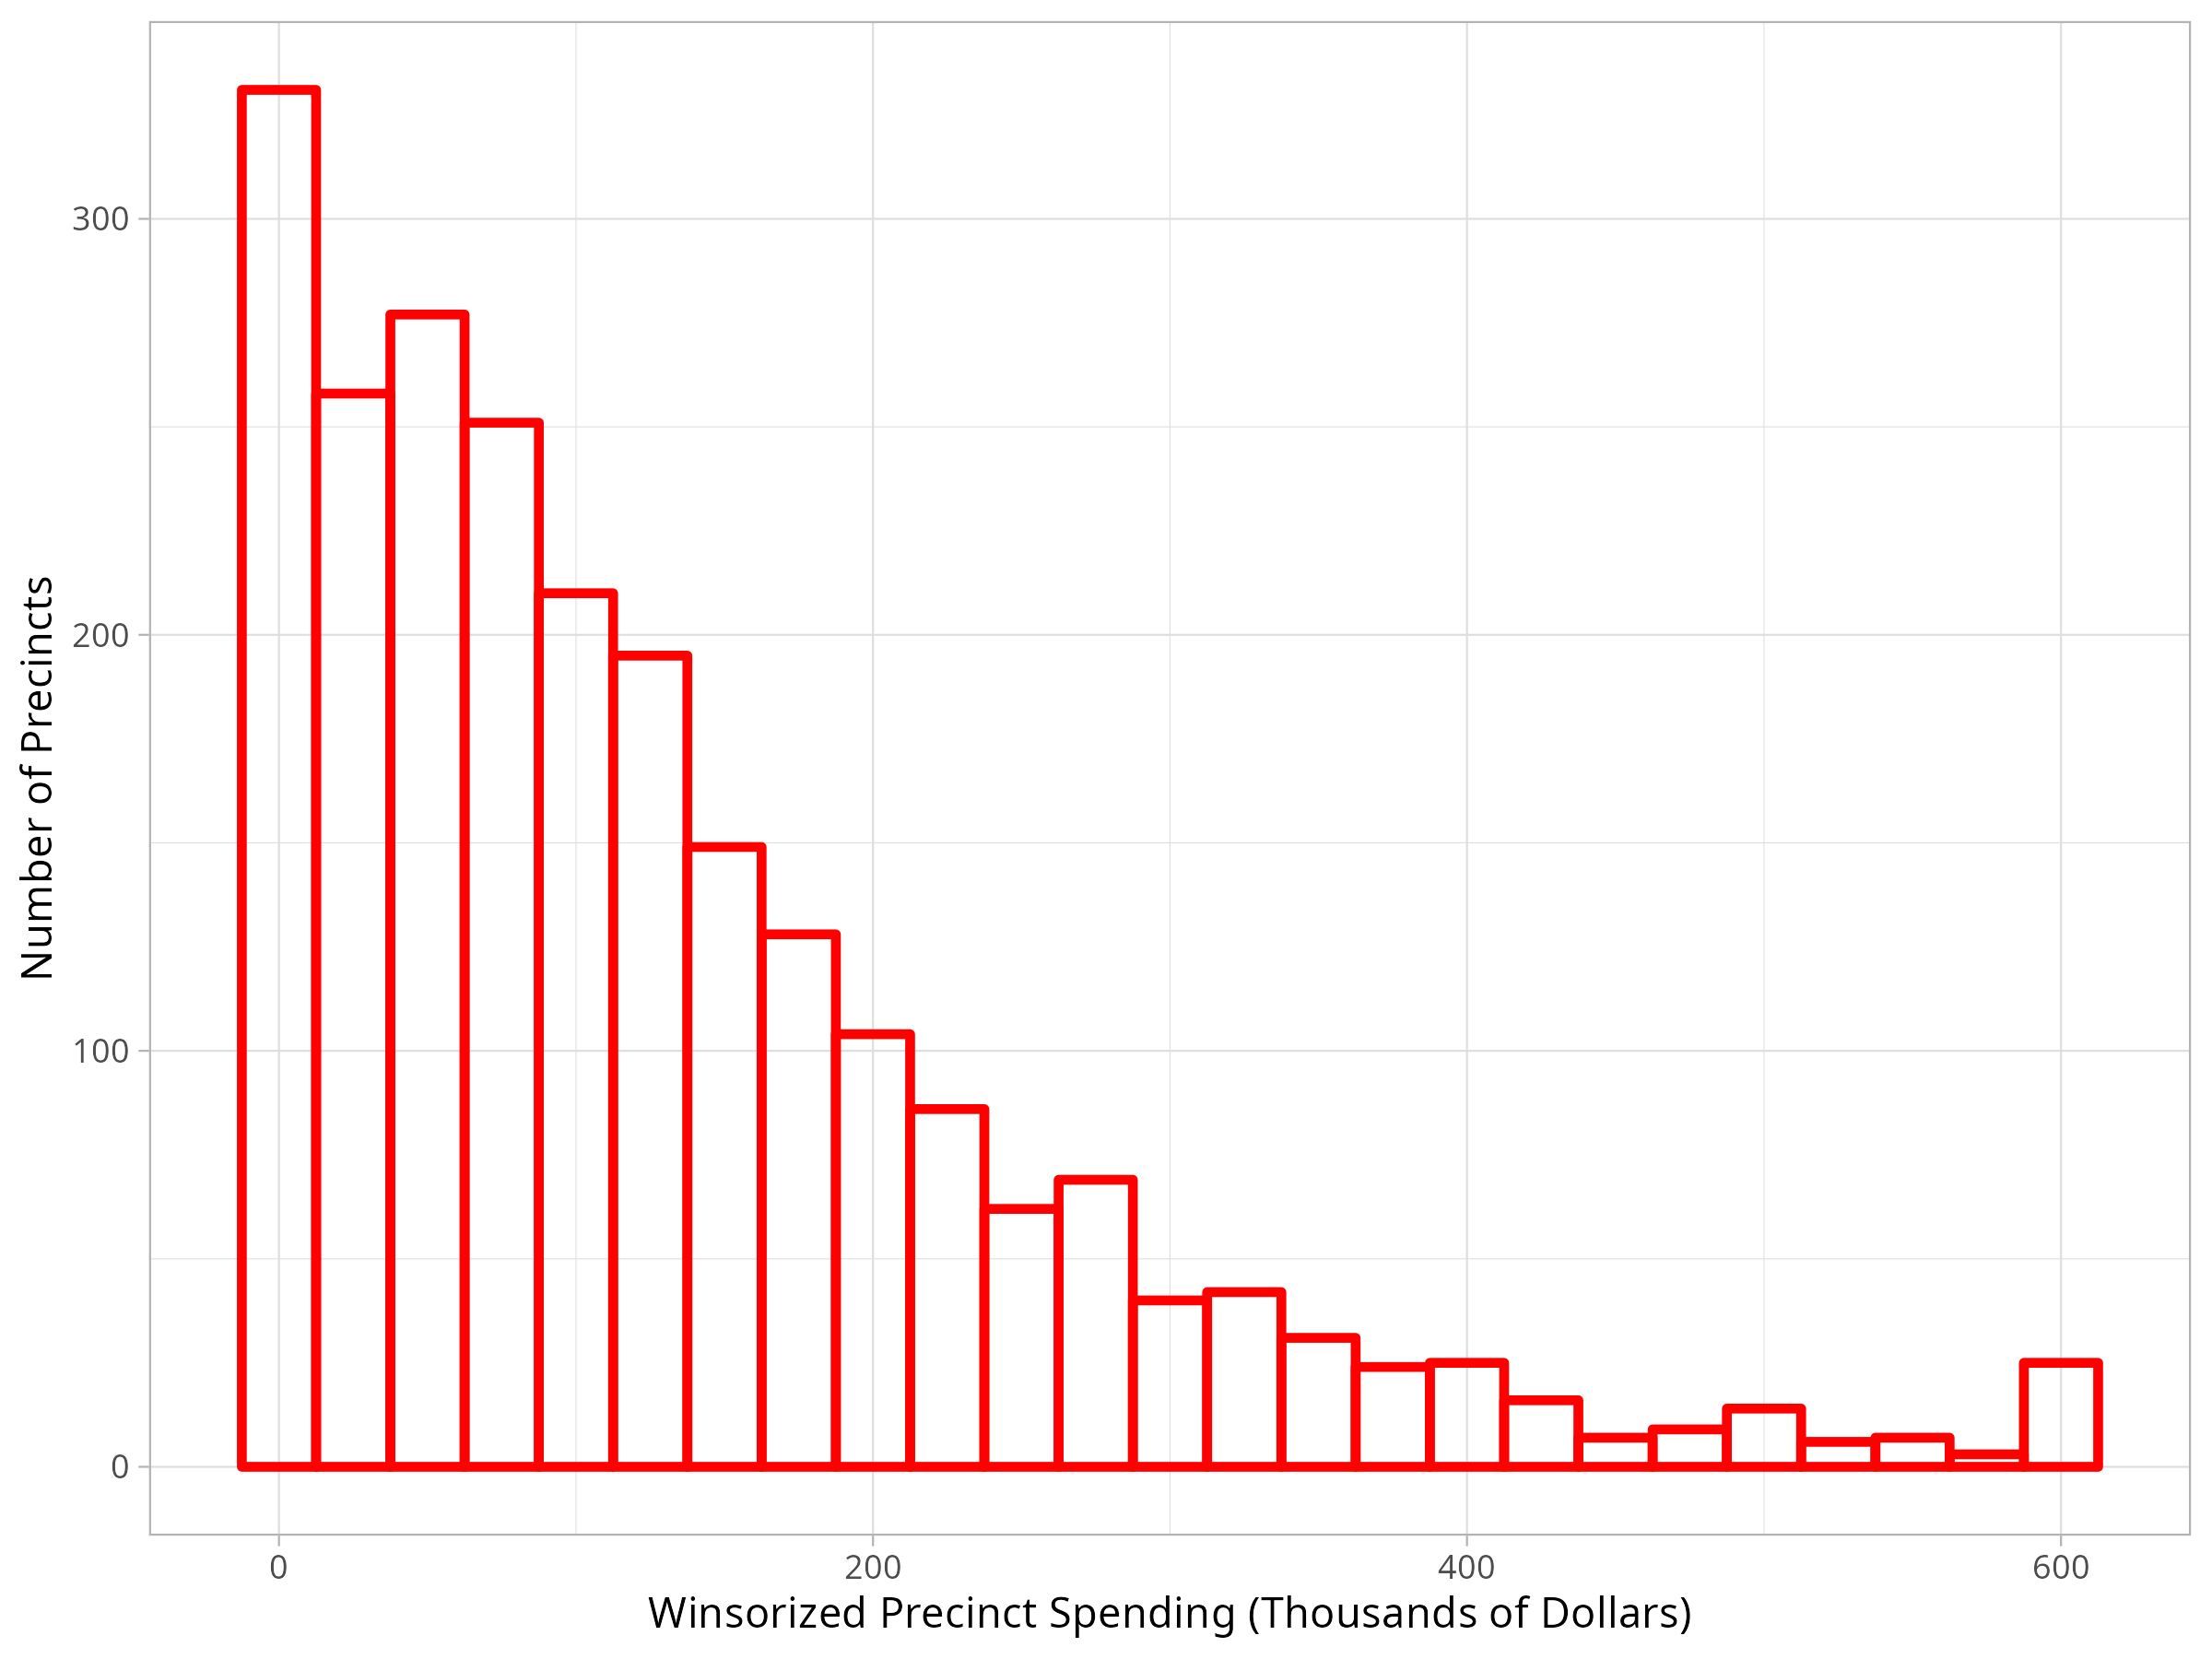
\includegraphics[width=\textwidth]{input/spending_histogram_2005_2011.png}
          \caption{Distribution of Spending per Precinct, 2005-2011}
          \label{fig:sub1}
        \end{subfigure}
        \hfill % This adds some space between the two subfigures
        % Second subfigure
        \begin{subfigure}[b]{0.45\textwidth}
          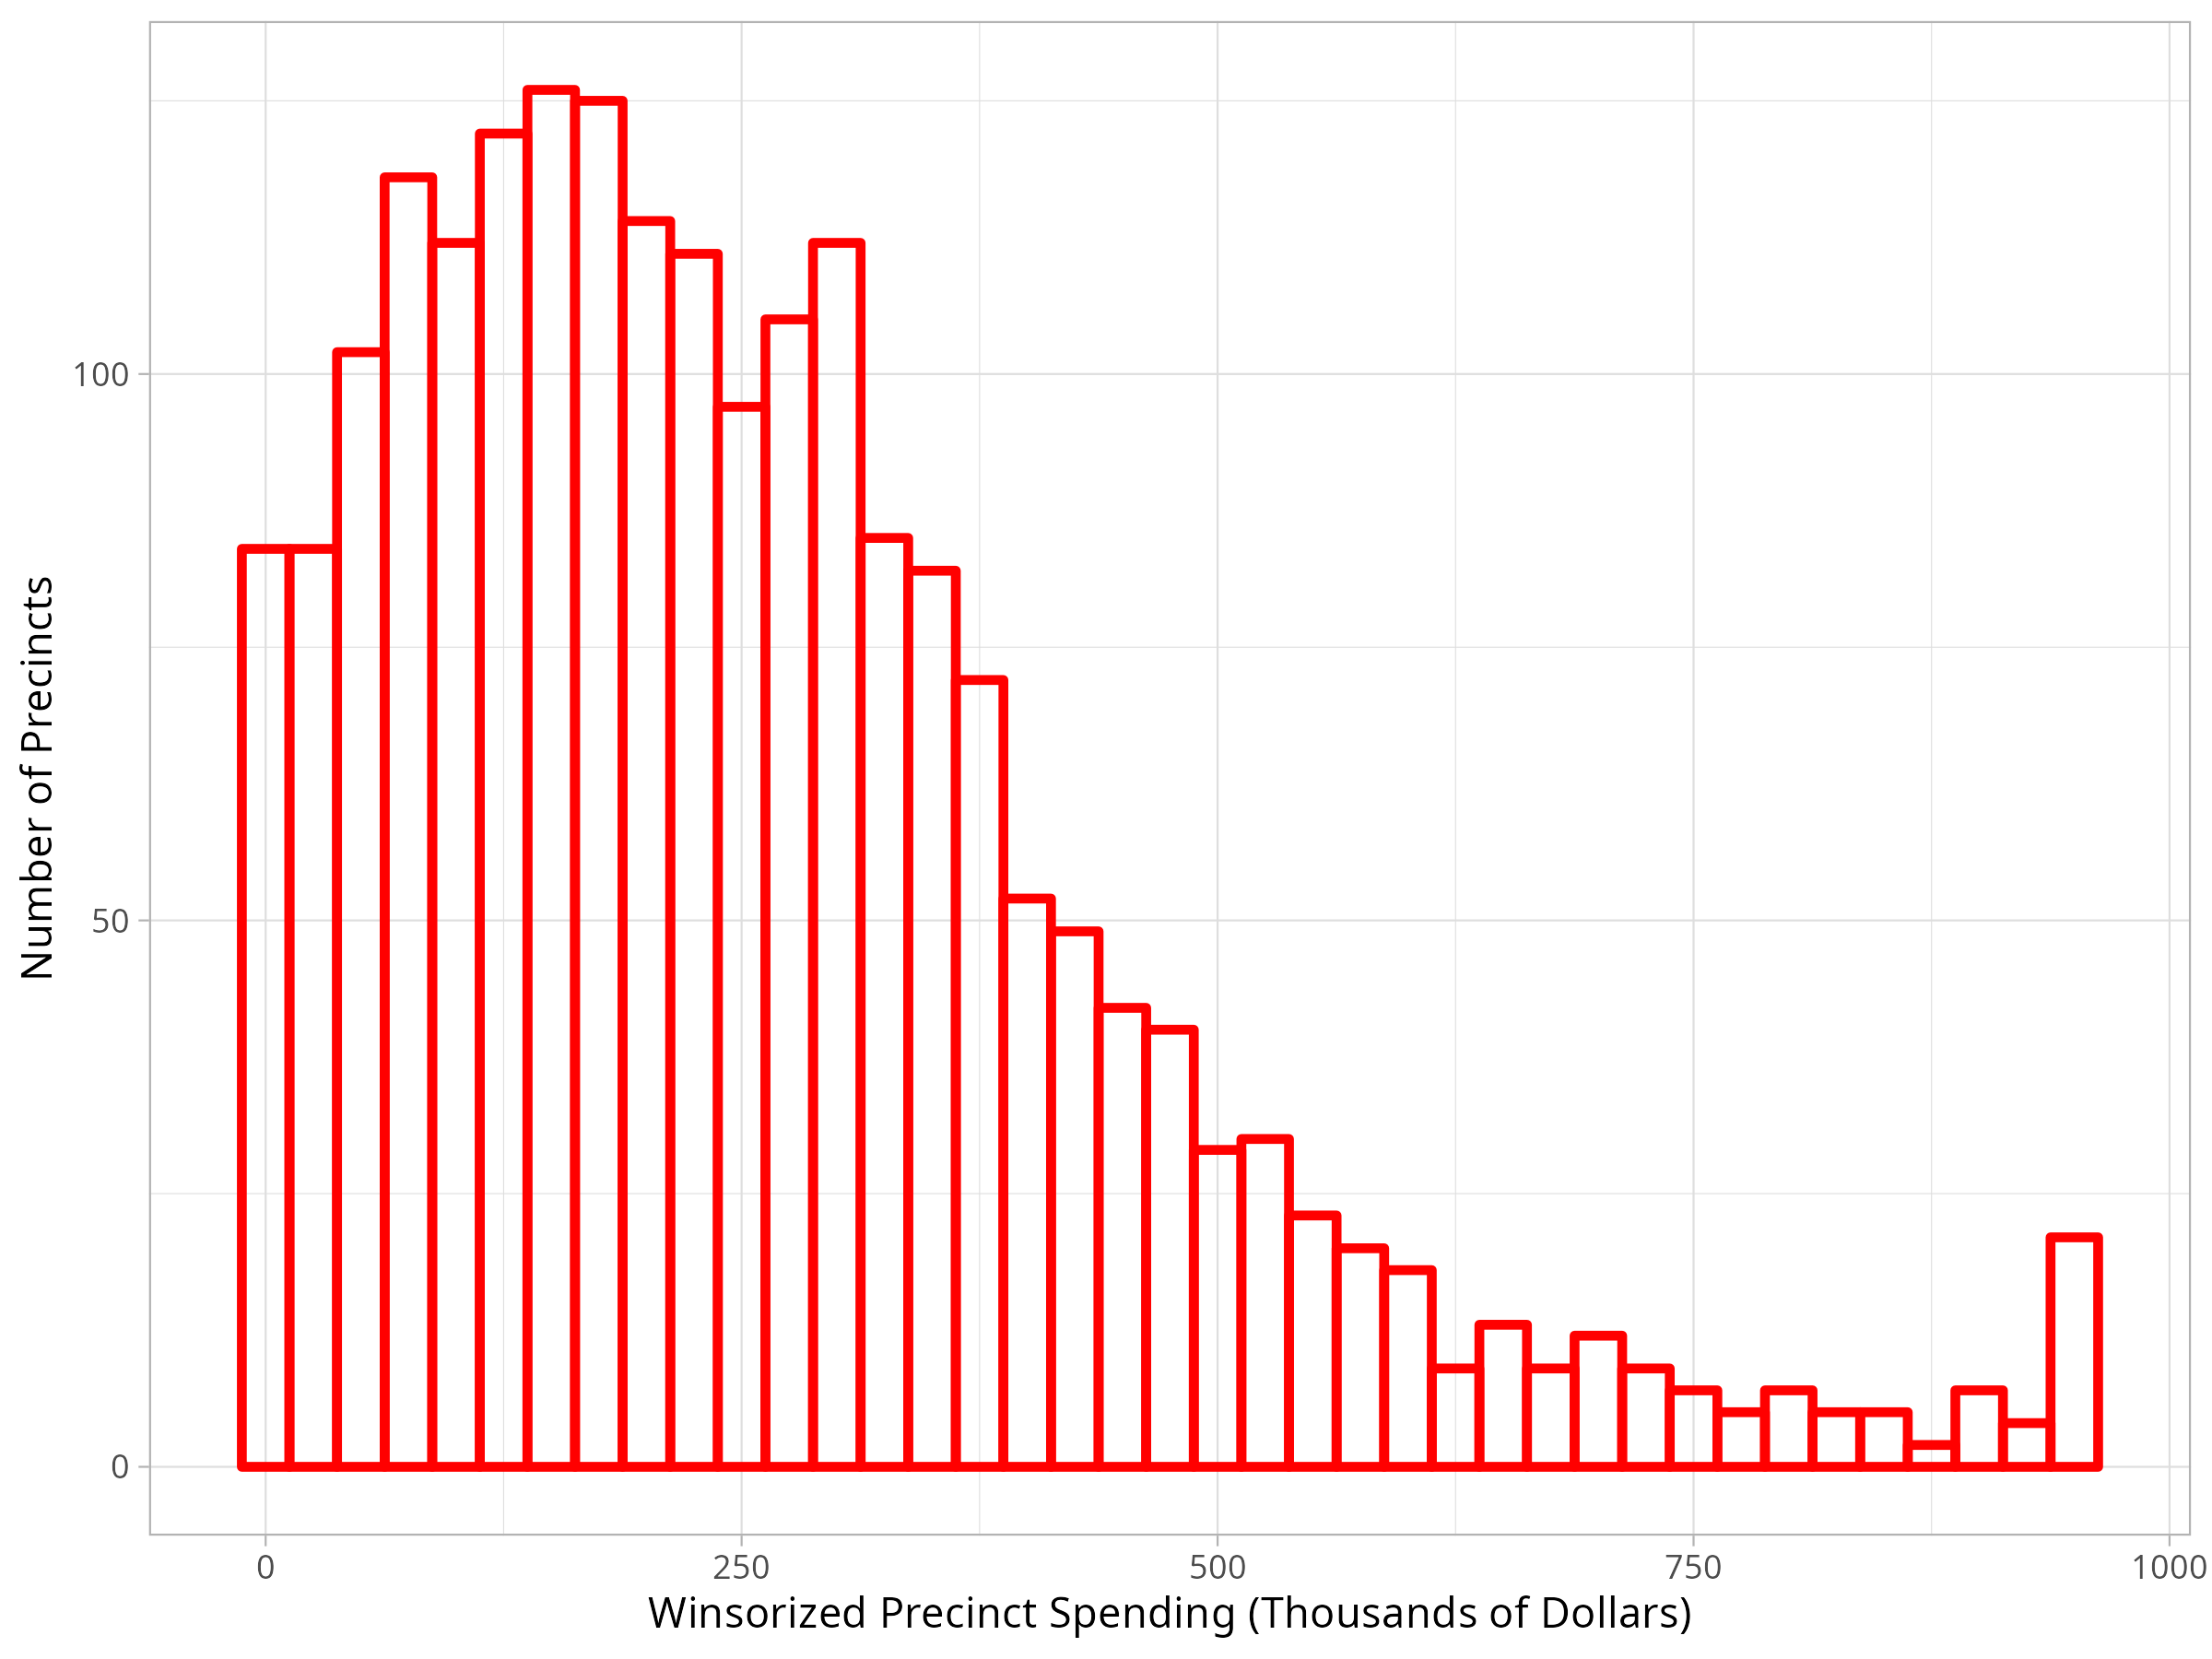
\includegraphics[width=\textwidth]{input/spending_histogram_2012_2022.png}
          \caption{Distribution of Spending per Precinct, 2012-2022}
          \label{fig:sub2}
        \end{subfigure}
      
        \caption{Distribution of Spending per Precinct for both ward maps in the dataset}
        \label{fig:spending_hist}
      \end{figure}
\end{frame}

\begin{frame}{Look at this cool map I made!}
    \begin{figure}[H]
        \centering
        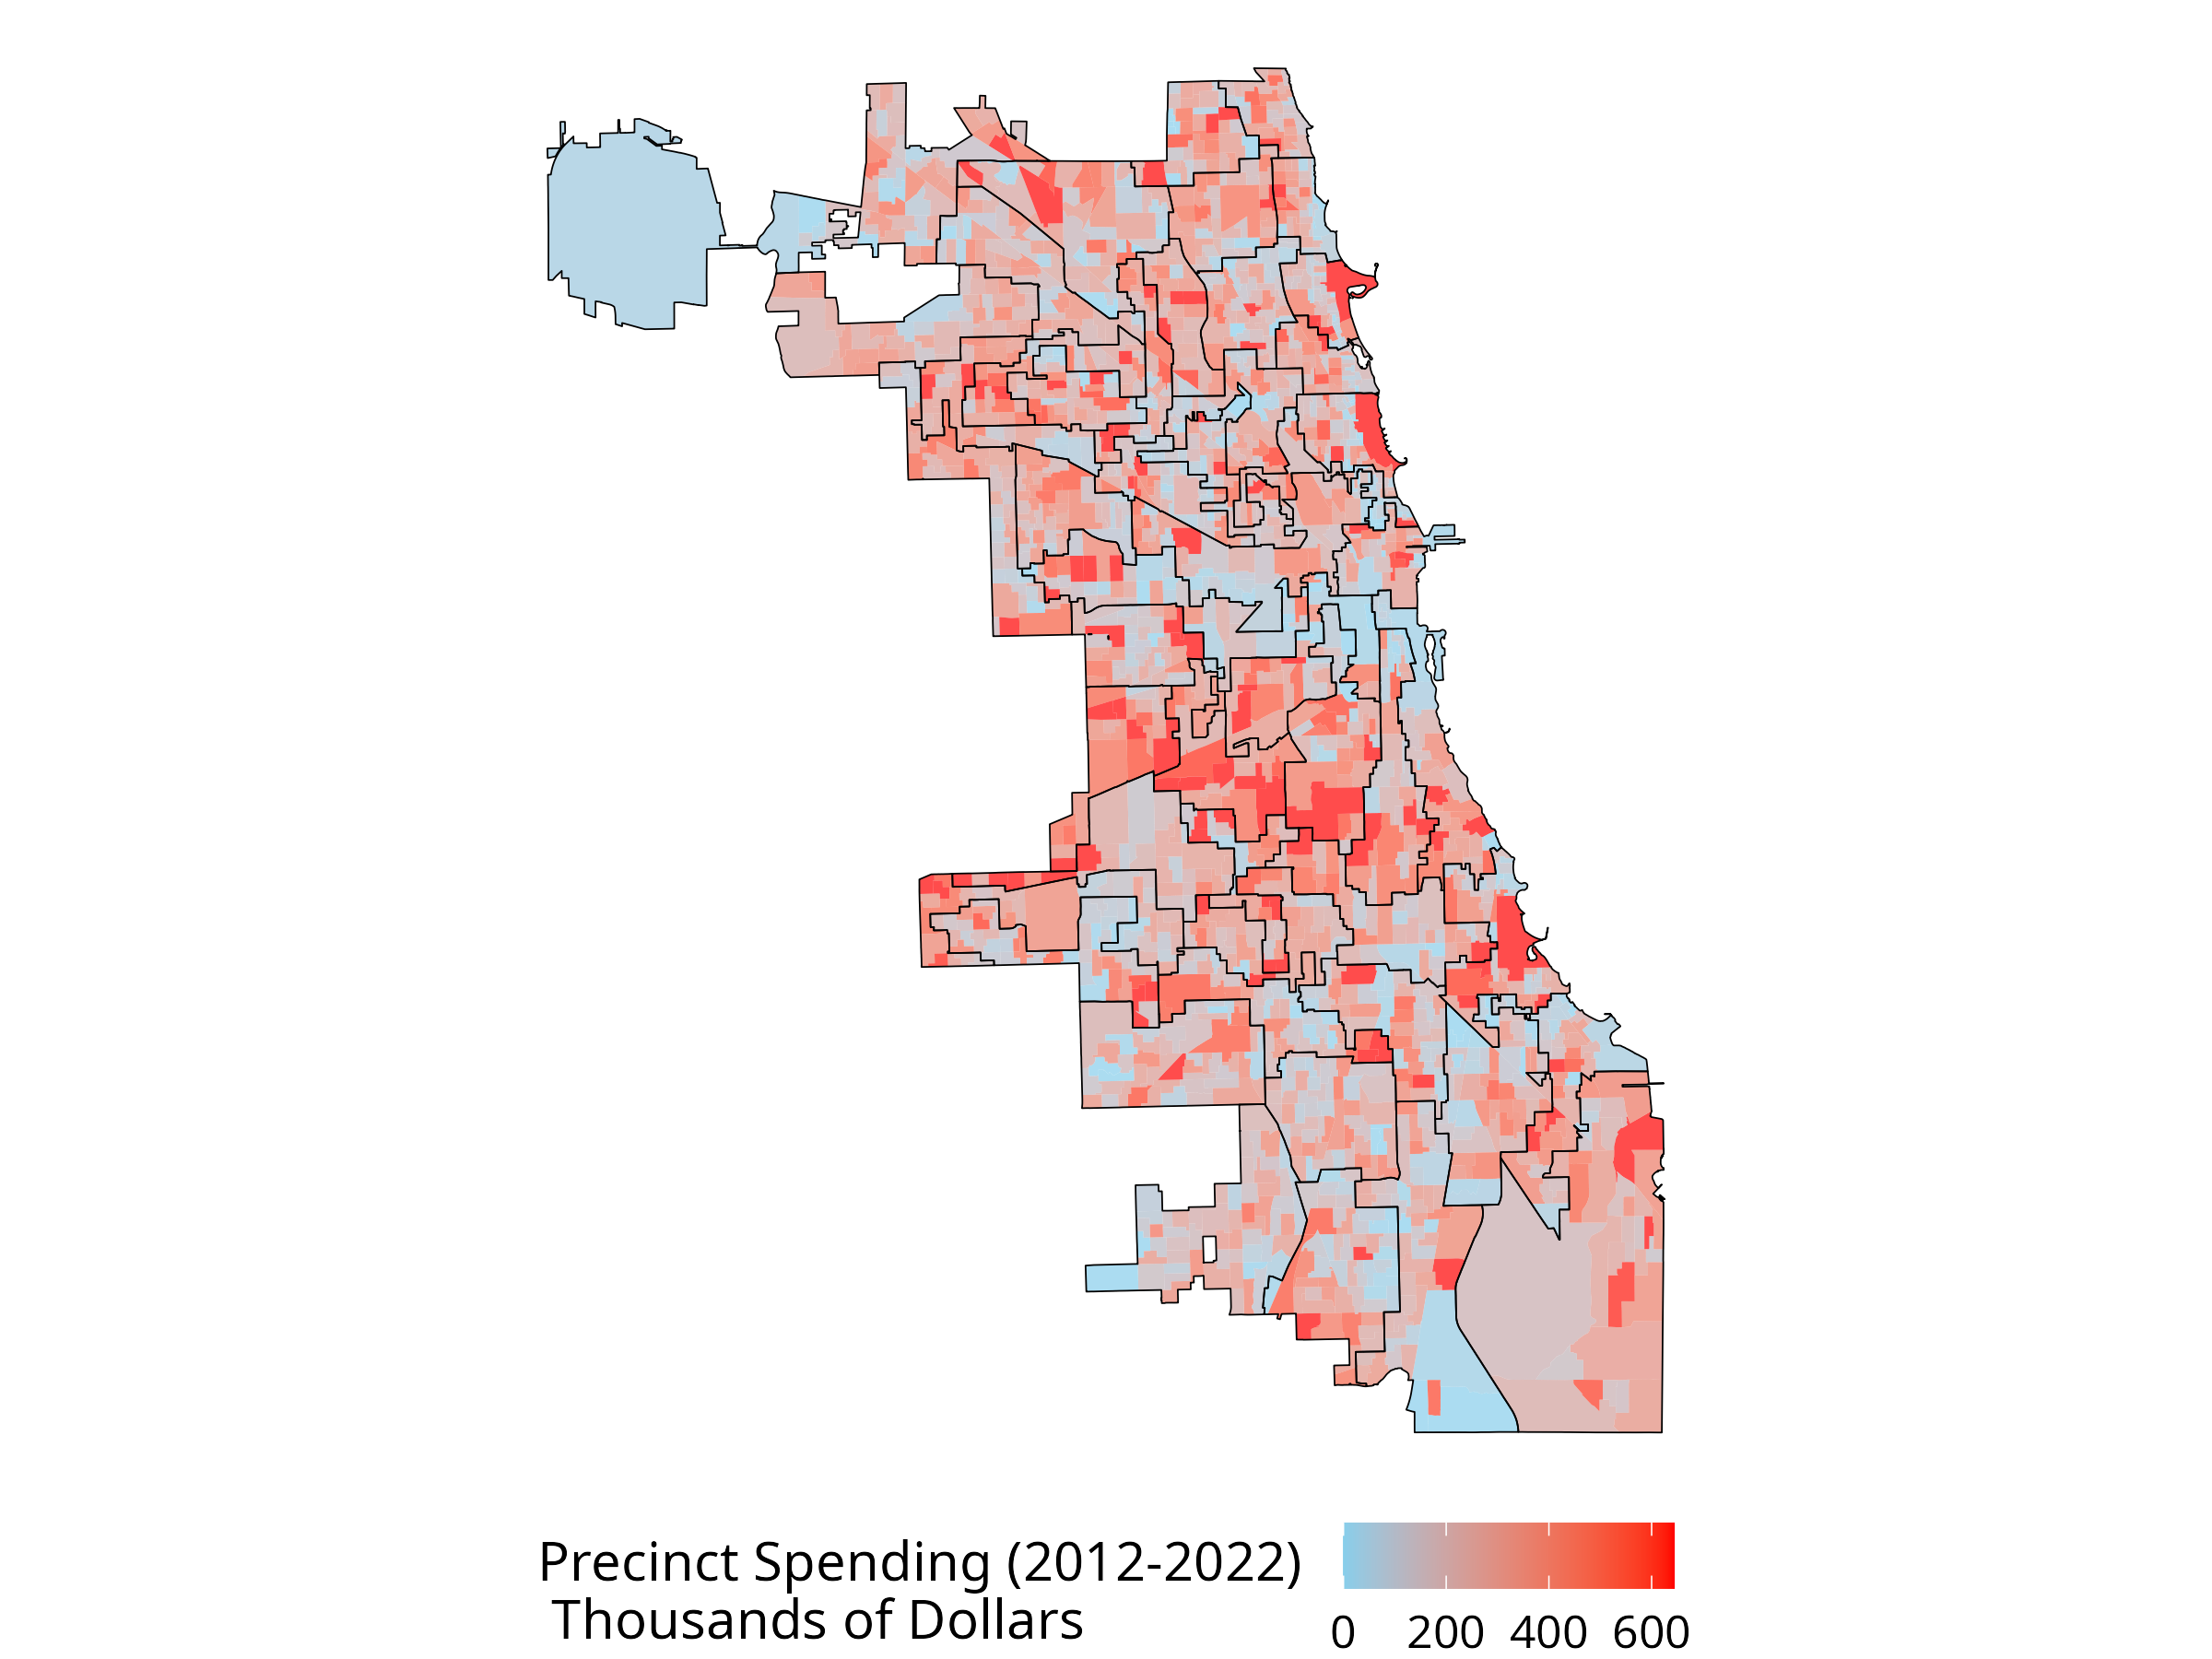
\includegraphics[width=0.6\textwidth]{input/whole_chicago_map_2012_2022.png}
        \caption{Map of Spending per Precinct, 2012-2022}
        \label{fig:spending_map}
    \end{figure}
\end{frame}